\chapter{Experimental Setup}

This chapter presents the experimental setup used to evaluate the task-
priority control framework developed in this thesis. It begins with an 
overview of the Eelume robot, including its mechanical structure, sensor suite
, communication systems, and suitability for underwater manipulation tasks. 
Following that, the software tools and interfaces used to control the robot 
and simulate its behavior are described. The chapter also outlines key 
assumptions and limitations in the experimental environment, including sensor 
noise and system constraints. Finally, the experimental procedures are detailed
, describing how specific robot behaviors will be tested and what kinds of 
responses are expected. Together, these sections provide the necessary context 
for understanding the practical validation of the proposed control approach.

% -----------------------------------------------------------------------------
\section{The Eelume Robot}

The Eelume \(500\) model M robot is a snake-like underwater vehicle developed by 
the company Eelume AS. It is designed for subsea inspection and light 
intervention tasks, and can be deployed in a variety of environments, 
including offshore wind farms, fish farms, and oil and gas installations. The 
system is highly modular, enabling a wide range of use cases.
The robot can operate either as an \gls{auv}, using an acoustic communication 
link, or as an \gls{rov} via a fiber-optic tether. A computer rendering of the 
Eelume robot is shown in \autoref{fig:eelume:stopdown}.

\begin{figure}[h!]
    \centering
    \includegraphics[width=\textwidth]{assets/ignored/s-topdown.png}
    \caption{A computer rendering of the Eelume robot configured in an S-shape.}
    \label{fig:eelume:stopdown}
\end{figure}

The Eelume robot can be equipped with a wide range of sensors, including a \gls{dvl},
\gls{imu}, \gls{uhi}, sonar, echo-sounder, fluorometer, \gls{ct}, and 
cameras. It uses an onboard \gls{ins} for navigation, supported by the \gls{dvl}
and an acoustic positioning system. At the surface, it is equipped with an 
antenna for satellite communication via Iridium, as well as \gls{gps}. Ballast 
modules allow for buoyancy control, enabling the robot to remain slightly 
positively buoyant in both fresh and salt water, depending on the configuration.
The onboard battery supports up to $8$ hours of operation, depending on 
usage and setup.

The configuration used in the experiments described in this thesis is similar 
to that shown in \autoref{fig:eelume:stopdown}, with some changes to module 
arrangement. The front of the robot is equipped with a \gls{uhi} instead of 
the forward-looking sonar shown in the figure. The overall shape, including 
thruster and joint placement, remains close to what is depicted. In this 
configuration, the Eelume robot weighs approximately $190$ kg and measures 
about $6.05$ m in length. From left to right in the image, we define the three 
links as \textit{tail}, \textit{body}, and \textit{head}, respectively. The 
following $5$ coordinate frames are attached to the robot:
\begin{itemize}
\item \textbf{tail} – the very end of the tail link, located on the left in \autoref{fig:eelume:stopdown}.
\item \textbf{tail center} – the center of the tail link.
\item \textbf{body} – the center of the body link.
\item \textbf{head center} – the center of the head link.
\item \textbf{head} – the very end of the head link, located on the right in \autoref{fig:eelume:stopdown}.
\end{itemize}

The $x$-axes of these frames align with the robot, pointing "forward." The $z$-
axes point downward toward the shadow, which also corresponds to the downward 
direction in \autoref{fig:eelume:stopdown}. The $y$-axes are defined by the 
right-hand rule. As the robot moves, the frames remain attached to their 
respective links and rotate with them. The coordinate frames at the centers of 
the head and tail links are useful for defining hydrodynamic damping forces, 
while the remaining three frames are primarily used for task definitions.

\begin{figure}[h!]
    \centering
    \begin{subfigure}{0.45\textwidth}
        \centering
        \includegraphics[width=\textwidth]{assets/ignored/s-1.png}
        \caption{The Eelume robot bending joints about the $z$-axis.}
        \label{fig:eelume:joints:1}
    \end{subfigure}
    \hfill
    \begin{subfigure}{0.45\textwidth}
        \centering
        \includegraphics[width=\textwidth]{assets/ignored/s-2.png}
        \caption{The Eelume robot bending joints about the $y$-axis.}
        \label{fig:eelume:joints:2}
    \end{subfigure}
    \caption{The Eelume robot with its two joints shown in different configurations.}
\label{fig:eelume:joints}
\end{figure}

The three links are connected by two joints, each with two degrees of freedom—
allowing rotation about both the $y$ and $z$ axes. \autoref{fig:eelume:joints} 
illustrates the joints in two different rotational configurations. The robot 
features two sets of $4$ thrusters: one set on the tail and another on the 
body link near the head joint. Each thruster can be independently controlled 
and provides bidirectional thrust. The thruster arrangement is shown in
\autoref{fig:eelume:thrusters}. When the robot is in a straight configuration, 
forces and moments can be generated independently in all $6$ \gls{dof}s. 
Together with the $2 \times 2$ \gls{dof}s from the joints, this results in a 
total of $10$ \gls{dof}s for this Eelume configuration. The joints are 
actuated by motors, bringing the total number of independent inputs to $12$:
$8$ thrusters and $4$ joint actuators.

The Eelume robot is an excellent platform for testing task-priority controllers
. This is largely due to its high number of \gls{dof}s, allowing for the 
execution of multiple tasks before kinematic constrains limit the robot. Additionally, 
the robot is highly coupled—motion in one link induces forces and moments in 
others. Task-priority control is an elegant approach for managing this coupling
, as the controller architecture inherently accommodates such interactions. In 
contrast, a typical large \gls{rov} with a manipulator arm exhibits minimal 
coupling, allowing the arm and vehicle to be controlled separately. In this 
respect, the Eelume robot is unique: it combines high \gls{dof} count with 
strong coupling, making it a compelling testbed for task-priority control.

% -----------------------------------------------------------------------------
\section{Tools and software}

The Eelume robot is controlled using a low-level \gls{api} that Eelume AS made
available in the beginning of 2025. This api provides access to low-level methods
for controlling the robot's thrusters and joints, as well as for reading sensor
data. The \gls{api} is implemented in C/C++ and communicates with the robot over
an ethernet connection. Because the \gls{api} is low-level, a lot of code had
to be written to implement the task-priority control framework, everyting from
lower-level controllers, task definitions, and kinematics. The collection of
code used to control the Eelume robot is created as a standalone C++ library
and is refered to as \gls{eck}.

The control kit is designed to be modular, allowing for easy integration of
new tasks and controllers. The library provides a set of virtual base classes,
one for a controller and one for a connection to the Eelume robot, along with
a set of concrete implementations for these classes. Setting and reading data
from the robot is done through the \gls{api} using a connection class, while 
a simulator is also provided for testing the controllers without the need for
a physical robot. Lower level \gls{dp} controllers, as well as higher-level
task-priority controllers are also implemented.

The simulator is designed to mimic the behavior of the Eelume robot as closely
as possible, without much time spent on modeling the hydrodynamics and coupling
between the links. The kinematics of the robot is tought to be accurately
implemented. Because of the virtual base classes, the real robot can be used
interchangeably without recompiling the code. This allows for easy testing of
the controllers after veryfing that they work in the simulator.

In addition to the control kit, the need for vizualization of the robot and
the tasks was identified. A simple visualizer was created to display the robot
in real time as experiments are conducted. The visualizer is implemented in
C++ using the OpenGL graphics library. The control kit communicates with the
visualizer over \gls{udp} sockets, sending the robot's state and task definitions.
Eelume robot that are presented in this thesis are created using this visualizer.
An example of the visualizer as it is used during experiments is shown in
\autoref{fig:eelume:visualizer}.

\begin{figure}[h!]
    \centering
    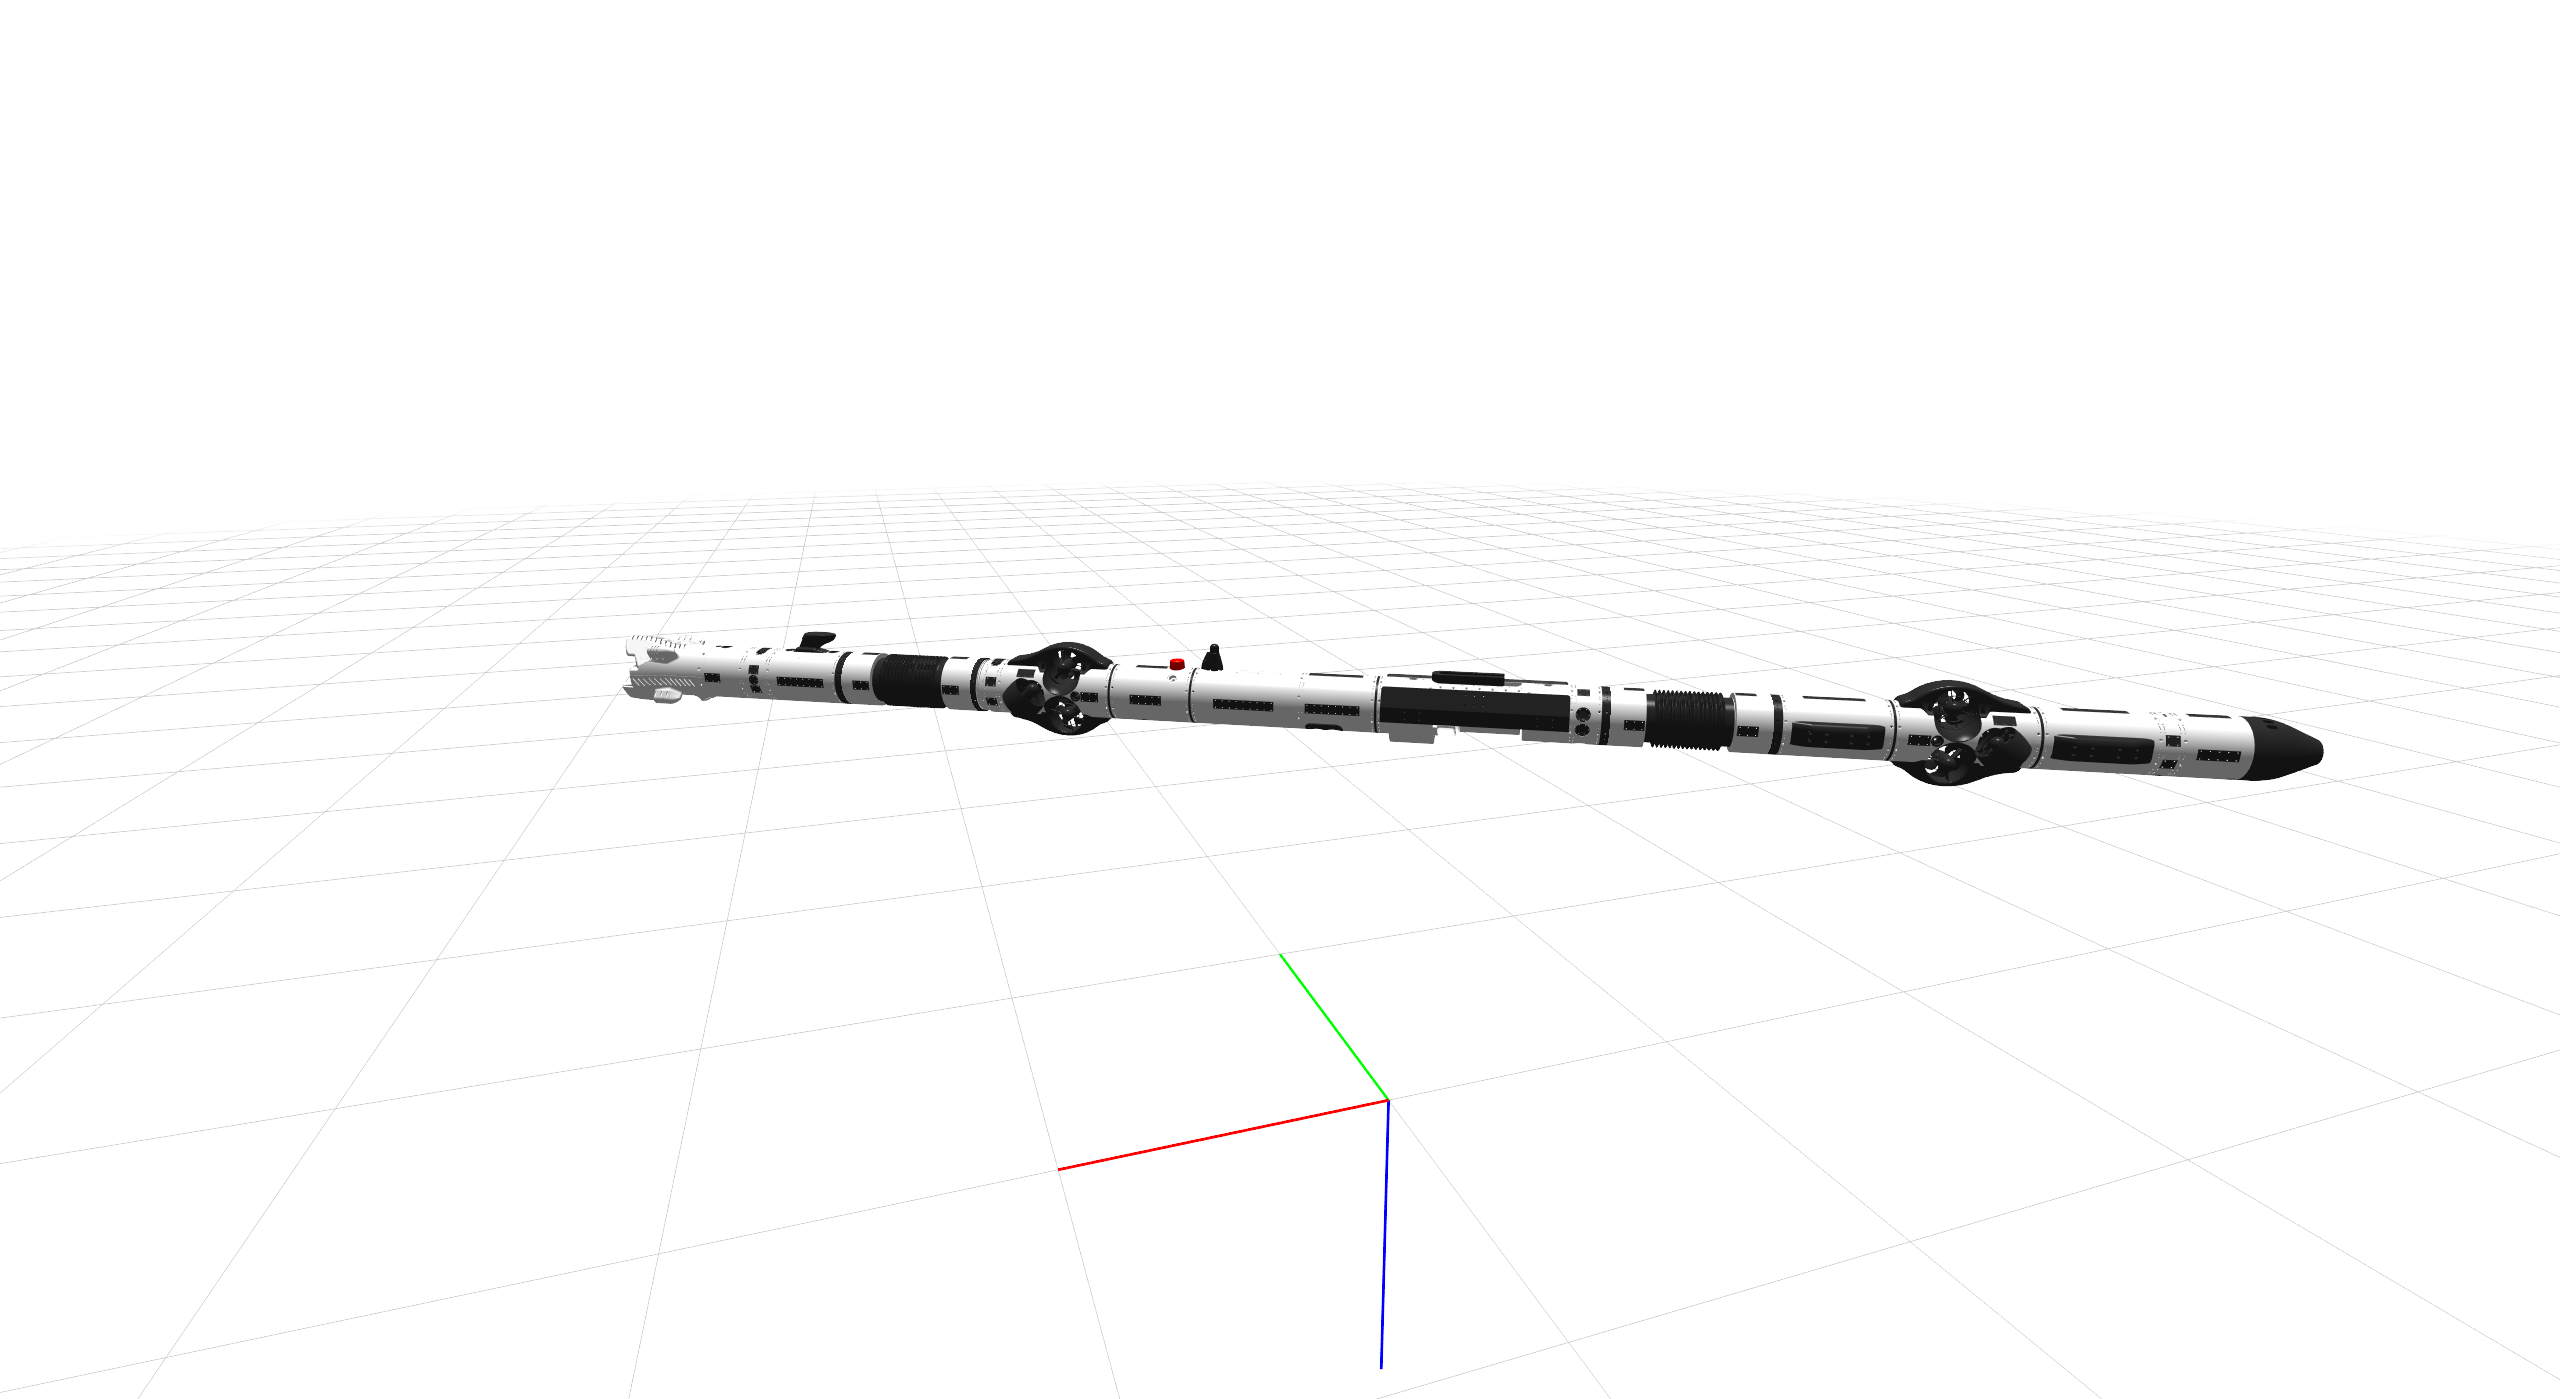
\includegraphics[width=\textwidth]{assets/eely-visualizer.png}
    \caption{A screenshot of the Eelume visualizer.}
    \label{fig:eelume:visualizer}
\end{figure}


%\begin{itemize}
%    \item the Eelume low-level api over ethernet
%    \item C/C++
%    \item developed simulator and connection to Eely
%    \item visualizer?
%\end{itemize}

% -----------------------------------------------------------------------------
\section{Assumptions and Limitations}
\begin{itemize}
    \item navigation system (jittery angles and noisy velocities)
    \item frequency limitations
    \item Topological limitations (cNode)
    \item roll rate limitations
    \item DVL bottom lock / accuracy in roll and pitch
    \item TBS, water depth and wave influence
    \item Don't know how well the thrusters/joint motors follows the reference.
\end{itemize}

The experiments are conducted at \gls{tbs} in the fjord outside Trondheim, Norway.
% -----------------------------------------------------------------------------
\section{Experimental Procedures}
\subsection*{Launch and test procedures}
\begin{itemize}
    \item Launch and test procedures
    \item show the response of the lower-level DP+ controller.
    \item Head + Tail stretching out
    \item Bending with joint constraints
    \item Expected results?
\end{itemize}

